% -*- root: Dissertation.tex -*-
\documentclass[Dissertation.tex]{subbIles}
\begin{document}
\graphicspath{{../Figures/}}
\chapter{Space-Time DPG for Incompressible Navier-Stokes}
\label{sec:incompressible}

\section{Introduction}
DPG for steady incompressible Navier-Stokes was studied by Roberts in \cite{NateDissertation}.
We choose a different variational formulation more consistent with 
our work with transient convection-diffusion.
The equations are trivial for one spatial dimension so space-time explorations of incompressible
Navier-Stokes require either 3D or 4D solves.
We derive a space-time DPG formulation for spatially 2D Navier-Stokes and show preliminary 
convergence results for the Taylor-Green vortex problem.

\section{Nonlinear Form}
The 2D incompressible Navier-Stokes equations are:
\begin{align*}
  \pd{\bfu}{t}+\Div\LRp{\bfu\otimes\bfu-\nu\Grad\bfu+p\bbI}&=\bff\\
  \Div\bfu&=0
  % \int_\Omega p&=0
\end{align*}
where $\bfu$ is the velocity, $p$ is the pressure, $\nu$ is the kinematic viscosity,
and $\bff$ contains any momentum source terms.
As a first order system in space-time divergence form, this is
\begin{align*}
  \frac{1}{\nu}\bbD-\Grad\bfu&=0\\
  \Divxt\vecttwo{\bfu\otimes\bfu-\bbD+p\bbI}{\bfu}&=\bff\\
  \Div\bfu&=0\,.
  % \int_\Omega p&=0
\end{align*}
Multiplying by test functions $\bbS\in\bbH(\text{div},Q)$, $\bfv\in\HonextQ$, $q\in\HonexQ$, 
and integrating by parts, we get
\begin{align*}
  \LRp{\frac{1}{\nu}\bbD,\bbS}
  +\LRp{\bfu,\Div\bbS}
  -\LRa{\hat\bfu,\bbS\cdot\bfn}&=0\\
  -\LRp{\vecttwo{\bfu\otimes\bfu-\bbD+p\bbI}{\bfu},\Gradxt\bfv}
  +\LRa{\hat\bft,\bfv}
  &=(\bff,\bfv)\\
  -\LRp{\bfu,\Grad q}
  +\LRa{\hat{\bfu}\cdot\bfn,q}&=0\,.
  % \int_\Omega p&=0
\end{align*}
where
\begin{align*}
\hat\bfu&=\trace(\bfu)\\
\hat\bft&=\trace\LRp{\bfu\otimes\bfu-\bbD+p\bbI}\cdot\bfn_x
+\trace(\bfu)\cdot n_t\,.
\end{align*}

\section{Linearization}
We split our residual into volume and trace terms:
\[
R(\bfu,p,\bbD,\hat\bfu,\hat\bft)=R(\bfu,p,\bbD)+R(\hat\bfu,\hat\bft)\,.
\]
where
\begin{align*}
R(\bfu,p,\bbD)=&
  \LRp{\frac{1}{\nu}\bbD,\bbS}
  +\LRp{\bfu,\Div\bbS}
  \\&
  -\LRp{\vecttwo{\bfu\otimes\bfu-\bbD+p\bbI}{\bfu},\Gradxt\bfv}
  -(\bff,\bfv)
  -\LRp{\bfu,\Grad q}
\end{align*}
and
\begin{align*}
R(\hat\bfu,\hat\bft)=
  -\LRa{\hat\bfu,\bbS\cdot\bfn}
  +\LRa{\hat\bft,\bfv}
  +\LRa{\hat{\bfu}\cdot\bfn,q}\,.
\end{align*}
Note that $R(\hat\bfu,\hat\bft)$ is already linear, so we only need to linearize terms dependent on 
the volume variables. Let 
$\LRc{\bfu,p,\bbD}=\LRc{\tilde\bfu,\tilde p,\tilde\bbD}+\LRc{\Delta\bfu,\Delta p,\Delta\bbD}$,
where $\LRc{\tilde\bfu,\tilde p,\bbD}$ is the previous solution in the Newton iteration 
and $\LRc{\Delta\bfu,\Delta p,\bbD}$ is the update.
We linearize about $\LRc{\tilde\bfu,\tilde p,\tilde\bbD}$ so that our linear problem becomes
\[
\pd{R(\tilde\bfu,\tilde p,\tilde\bbD)}{(\bfu,p,\bbD)}\vectthree{\Delta\bfu}{\Delta p}{\Delta\bbD}+R(\hat\bfu,\hat\bft)
=-R(\tilde\bfu,\tilde p,\tilde\bbD)
\]
where 
\begin{align*}
\pd{R(\tilde\bfu,\tilde p,\tilde\bbD)}{(\bfu,p,\bbD)}\vectthree{\Delta\bfu}{\Delta p}{\Delta\bbD}=
  \LRp{\frac{1}{\nu}\Delta\bbD,\bbS}
  +\LRp{\Delta\bfu,\Div\bbS}
  \\
  -\LRp{\vecttwo{\Delta\bfu\otimes\tilde\bfu+\tilde\bfu\otimes\Delta\bfu-\Delta\bbD+\Delta p\bbI}
  {\Delta\bfu},\Gradxt\bfv}
  \\
  -\LRp{\Delta\bfu,\Grad q}\,.
\end{align*}

Note that for the steady state case, the pressure is only uniquely defined up to a constant
so in order to obtain a unique solution it is sufficient to set either a zero mean condition
or to constrain the pressure to a certain value at a point.
In the transient case, pressure is unique up to any arbitrary function of $t$.
This issue disappears for problems with boundary conditions on $\hat\bft$ as the definition 
of the flux contains a pressure term, but for problems with pure $\hat\bfu$ boundary conditions,
we choose a spatial point and constrain the pressure to a specific value at that point for all time.

\section{Robust Test Norms}
We develop test norms for the incompressible Navier-Stokes equations by drawing analogies to our
robust norms for transient convection-diffusion. 
If we group the test terms according to their interaction with trial variables, 
the left hand side of the convection-diffusion bilinear form looks like:
\begin{equation*}
  (\bfsigma,\frac{1}{\epsilon}\bftau+\Grad v)+(u,\Div\bftau-\bfbeta\cdot\Grad v-\pd{v}{t})\,.
\end{equation*}
Doing the same thing for incompressible Navier-Stokes yields:
\begin{align*}
  \LRp{\Delta\bbD,\frac{1}{\nu}\bbS+\Grad\bfv}
  &+\LRp{\Delta\bfu,\Div\bbS-\Grad q-\LRp{\tilde\bfu\cdot\Grad\bfv +\tilde\bfu\cdot(\Grad\bfv)^T+\pd{\bfv}{t}}}
  \\&+\LRp{p,-\Div\bfv}\,.
\end{align*}
Recall the robust \eqref{eq:meshrobustnorm} and coupled robust \eqref{eq:meshcoupledrobustnorm} test norms:
\begin{align*}
\norm{\LRp{v,\bftau}}_{V,K}^2 &\coloneqq
\norm{\bfbeta\cdot\Grad v+\pd{v}{t}}_K^2
+ \epsilon\norm{\Grad v}_K^2
+ \min\LRp{\frac{\epsilon}{h^2},1}\norm{v}^2_K
\\\nonumber&\quad
+ \norm{\Div \bftau}_K^2
+ \min\LRp{\frac{1}{\epsilon},\frac{1}{h^2}}\norm{\bftau}_K^2\,,
\end{align*}
and
\begin{align*}
\norm{\LRp{v,\bftau}}_{V,K}^2 &\coloneqq
\norm{\bfbeta\cdot\Grad v+\pd{v}{t}}_K^2
+ \epsilon\norm{\Grad v}_K^2
+ \min\LRp{\frac{\epsilon}{h^2},1}\norm{v}^2_K
\\\nonumber&\quad
+ \norm{\Div \bftau - \bfbeta\cdot\Grad v-\pd{v}{t}}_K^2
+ \min\LRp{\frac{1}{\epsilon},\frac{1}{h^2}}\norm{\bftau}_K^2\,.
\end{align*}
This leads us to define the respective norms for incompressible Navier-Stokes:
\begin{align*}
\norm{\LRp{\bfv,\bbD,q}}_{V,K}^2 &\coloneqq
\norm{\tilde\bfu\cdot\Grad\bfv +\tilde\bfu\cdot(\Grad\bfv)^T+\pd{\bfv}{t}}_K^2
+ \nu\norm{\Grad\bfv}_K^2
+ \min\LRp{\frac{\nu}{h^2},1}\norm{\bfv}^2_K
\\\nonumber&\quad
+ \norm{\Div\bbS-\Grad q}_K^2
\\\nonumber&\quad
+ \min\LRp{\frac{1}{\nu},\frac{1}{h^2}}\norm{\bbS}_K^2
+\norm{\Div\bfv}_K^2
+\norm{q}_K^2
\,,
\end{align*}
and
\begin{align*}
\norm{\LRp{\bfv,\bbD,q}}_{V,K}^2 &\coloneqq
\norm{\tilde\bfu\cdot\Grad\bfv +\tilde\bfu\cdot(\Grad\bfv)^T+\pd{\bfv}{t}}_K^2
+ \nu\norm{\Grad\bfv}_K^2
+ \min\LRp{\frac{\nu}{h^2},1}\norm{\bfv}^2_K
\\\nonumber&\quad
+ \norm{\Div\bbS-\Grad q-\LRp{\tilde\bfu\cdot\Grad\bfv +\tilde\bfu\cdot(\Grad\bfv)^T+\pd{\bfv}{t}}}_K^2
\\\nonumber&\quad
+ \min\LRp{\frac{1}{\nu},\frac{1}{h^2}}\norm{\bbS}_K^2
+\norm{\Div\bfv}_K^2
+\norm{q}_K^2
\,.
\end{align*}
% We haven't developed a mathematical theory for it, but we've also had numerical success with a norm that 
% we've dubbed the NSDecoupled norm because we first stumbled on it during experiements with compressible
% Navier-Stokes.
% The version for convection-diffusion looks like:
% \begin{align*}
% \norm{\LRp{v,\bftau}}_{V,K}^2 &\coloneqq
% \norm{\bfbeta\cdot\Grad v+\pd{v}{t}}_K^2
% + \norm{\Grad v}_K^2
% + \norm{v}^2_K
% \\\nonumber&\quad
% + \norm{\Div \bftau}_K^2
% + \frac{1}{h^2}\norm{\bftau}_K^2\,,
% \end{align*}
% and the analogous incompressible Navier-Stokes norm:
% \begin{align*}
% \norm{\LRp{\bfv,\bbD,q}}_{V,K}^2 &\coloneqq
% \norm{\tilde\bfu\cdot\Grad\bfv +\tilde\bfu\cdot(\Grad\bfv)^T+\pd{\bfv}{t}}_K^2
% + \norm{\Grad\bfv}_K^2
% + \norm{\bfv}^2_K
% \\\nonumber&\quad
% + \norm{\Div\bbS-\Grad q}_K^2
% \\\nonumber&\quad
% + \frac{1}{h^2}\norm{\bbS}_K^2
% +\norm{\Div\bfv}_K^2
% +\norm{q}_K^2
% \,.
% \end{align*}

\section{Numerical Experiments}
\subsection{Taylor-Green Vortex}
% This is one of the few transient incompressible Navier-Stokes problems with an analytical solution.
The problem domain is $[0,2\pi]\times[0,2\pi]$ with a final time of $\pi$ and the analytical solution is 
\[
\bfu=e^{-\frac{2}{Re}t}\vecttwo{\sin{x}\cos{y}}{-\cos{x}\sin{y}}\,,
\]
a vector plot of which is shown in Figure \ref{fig:TaylorGreenVortex}.
We apply spatial boundary conditions on $\hat\bfu$ and at $t=0$ we apply boundary conditions
on $\hat\bft$ according to the initial conditions.
Plots of $L^2$ and energy ($V^*$) error for various polynomial orders and Reynolds numbers are shown
in Figure \ref{fig:TaylorGreenConvergence} for the coupled robust norm.

\begin{figure}
\centering
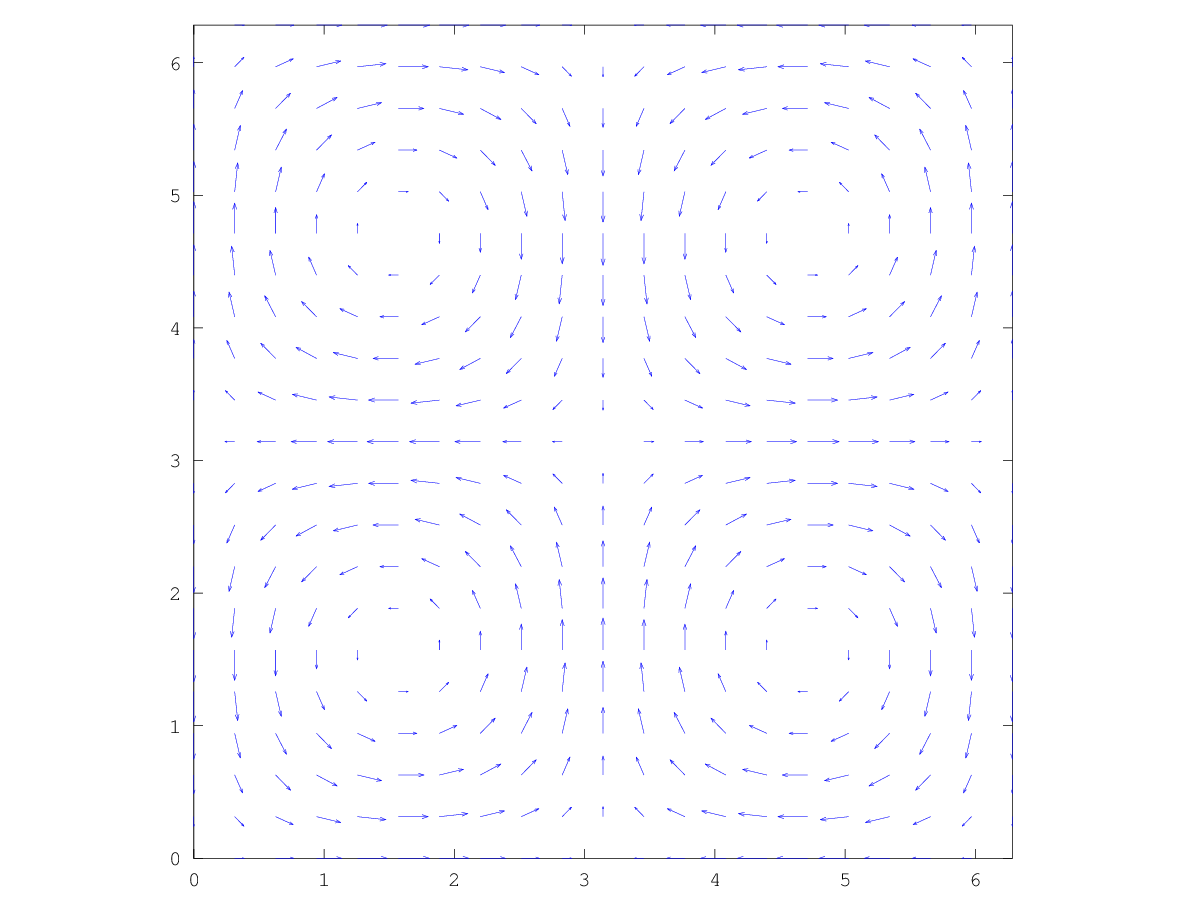
\includegraphics[width=0.8\textwidth]{Incompressible/TaylorGreen/Taylor-Green_vortex_vector_plot.png}
\caption{Taylor-Green vortex}
\label{fig:TaylorGreenVortex}
\end{figure}

\begin{figure}
\centering
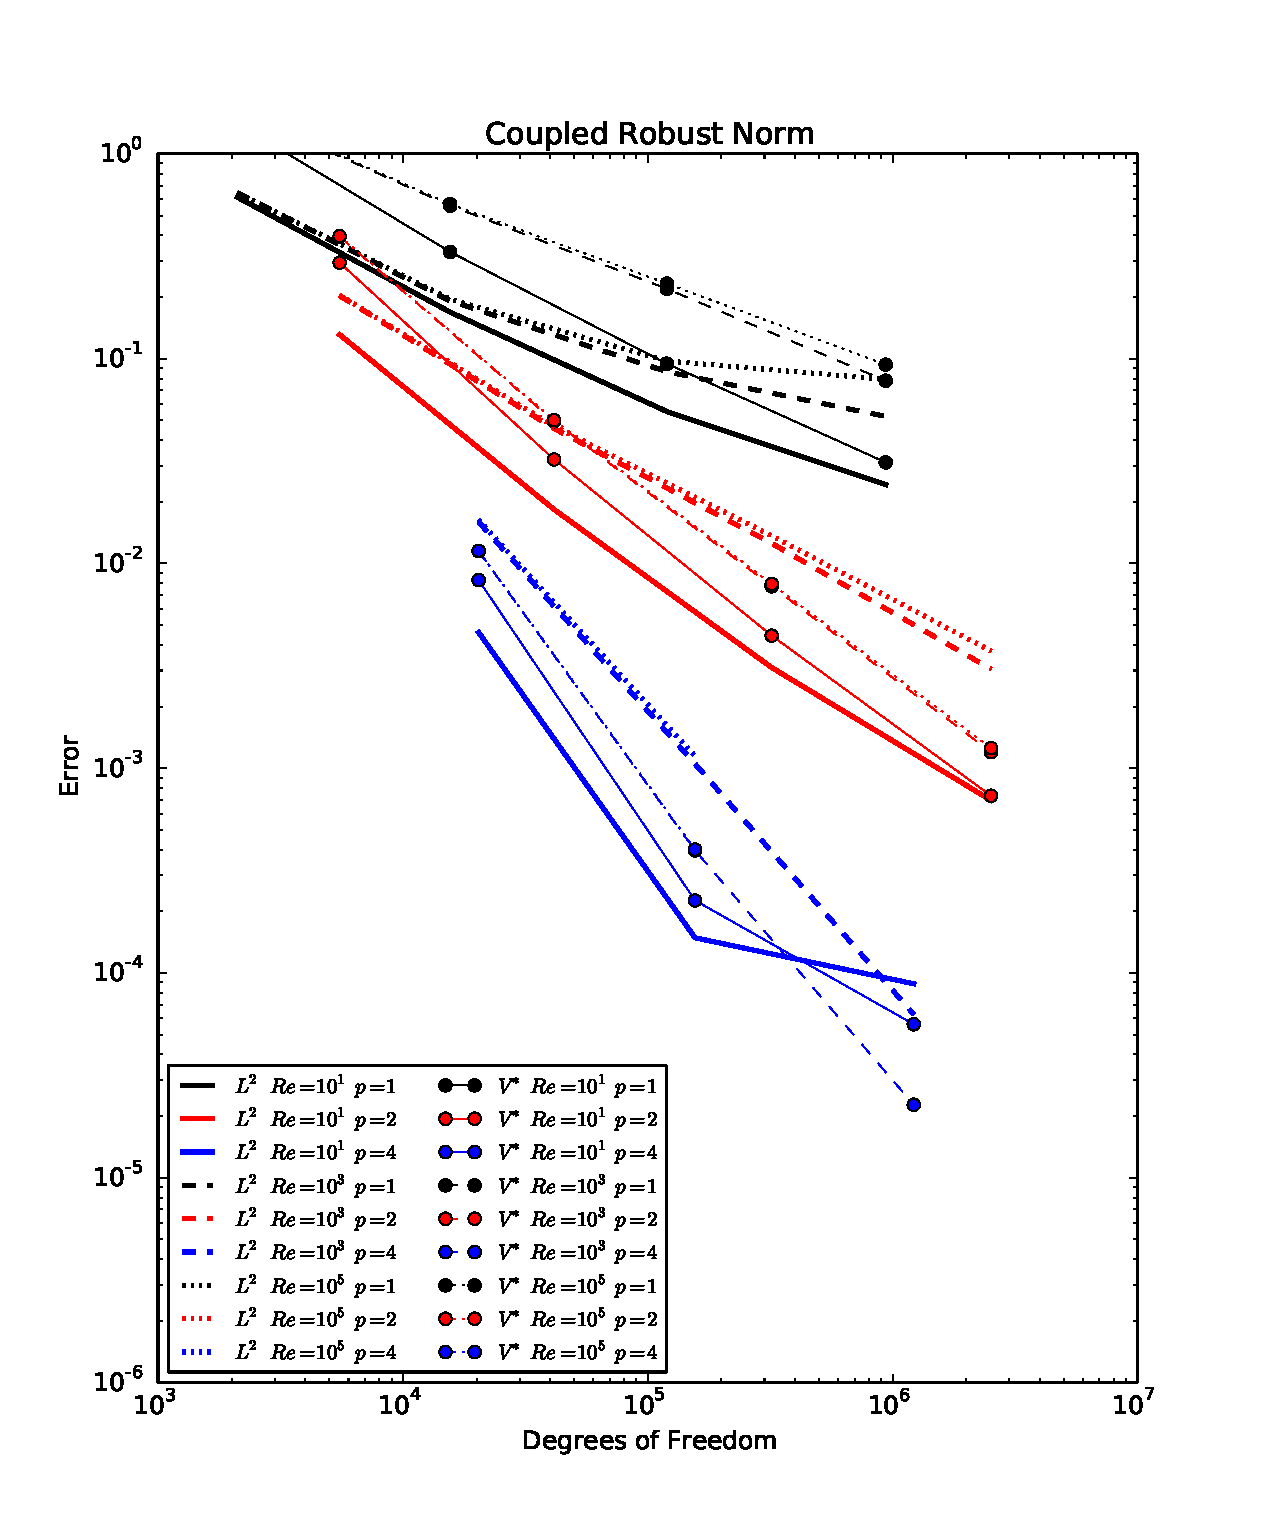
\includegraphics[width=\textwidth]{Incompressible/TaylorGreen/coupledrobust_convergence.pdf}
\caption{Convergence to Taylor-Green analytical solution}
\label{fig:TaylorGreenConvergence}
\end{figure}

\end{document}
